\section{Các cơ chế tích hợp hệ thống}
\label{sec:tich_hop_he_thong}

MyHCMUT Mobile khai thác chức năng từ các hệ thống hiện hữu thông qua API và một số cơ chế tích hợp phục vụ thiết bị di động. Mục này trình bày cách ứng dụng phối hợp với Auth Service, HRM Backend, iOffice Backend và các thành phần liên quan trong quá trình xác thực, chuyển tiếp phiên làm việc, tiếp nhận thông báo và tổng hợp dữ liệu nghiệp vụ.

\subsection{Xác thực và giao tiếp API}
\label{subsec:xac_thuc_da_he_thong}

Ứng dụng sử dụng Auth Service hiện hữu để đăng nhập và nhận access token. Sau khi đăng nhập thành công, token được ứng dụng quản lý và sử dụng khi gửi yêu cầu đến các backend nghiệp vụ. MyHCMUT Mobile tạo các Dio instance theo địa chỉ của từng dịch vụ; mỗi instance được cấu hình sẵn khóa xác thực (\texttt{domainKey}) để xác định token cần sử dụng.

Trong phiên bản hiện tại, các Dio instance phục vụ Auth Service, HRM Backend và iOffice Backend đều sử dụng chung khóa \texttt{auth}. Vì vậy, ứng dụng tái sử dụng cùng access token do Auth Service cấp, không quản lý ba token độc lập. Khi gửi yêu cầu cần xác thực, \texttt{MultiDomainAuthInterceptor} đọc token theo khóa đã cấu hình và gắn vào HTTP header theo dạng \texttt{Authorization: Bearer <token>}.

HRM Backend và iOffice Backend tiếp nhận yêu cầu, xác thực token và kiểm tra quyền truy cập đối với chức năng nghiệp vụ tương ứng. Ứng dụng di động quản lý phiên đăng nhập và gửi thông tin xác thực; các quyết định phân quyền và xử lý dữ liệu chính thức vẫn thuộc trách nhiệm của backend.

\subsection{Chuyển tiếp phiên làm việc sang HRM Web}
\label{subsec:sso_bridge}

Một số biểu mẫu hồ sơ được cung cấp thông qua HRM Web và được mở từ ứng dụng bằng WebView. Để người dùng không phải đăng nhập lại, hệ thống sử dụng vé xác thực dùng một lần (\textit{One-Time Ticket SSO}) nhằm chuyển tiếp từ phiên đăng nhập trên mobile sang phiên làm việc trên HRM Web mà không đưa access token hoặc refresh token lên URL.

Khi người dùng yêu cầu mở biểu mẫu, ứng dụng gửi yêu cầu đến endpoint \texttt{POST /api/auth/sso/generate-ticket} của HRM Backend. Backend tạo vé xác thực dùng một lần và lưu bản ghi tương ứng trong Redis với thời hạn 60 giây. Payload gắn với vé chứa mã cán bộ, hệ thống đích và thời điểm tạo. Khi tiêu thụ vé, HRM Backend chỉ chấp nhận bản ghi có \texttt{targetSystem} tương ứng với HRM. Backend trả vé cho ứng dụng; WebView mở địa chỉ biểu mẫu HRM Web kèm vé. HRM Web gửi vé trong nội dung yêu cầu đến endpoint \texttt{POST /api/auth/sso/consume-ticket}. HRM Backend dùng thao tác \texttt{GETDEL} của Redis để lấy và xóa vé trong cùng một thao tác; nếu vé hợp lệ, backend tạo và lưu phiên Web mới. Trong quá trình xử lý chuyển tiếp phiên, HRM Web sử dụng \texttt{history.replaceState} để loại bỏ tham số \texttt{ticket} khỏi URL. Toàn bộ luồng chuyển tiếp phiên làm việc được minh họa trong Hình~\ref{fig:sso_sequence}.

\begin{figure}[H]
    \centering
    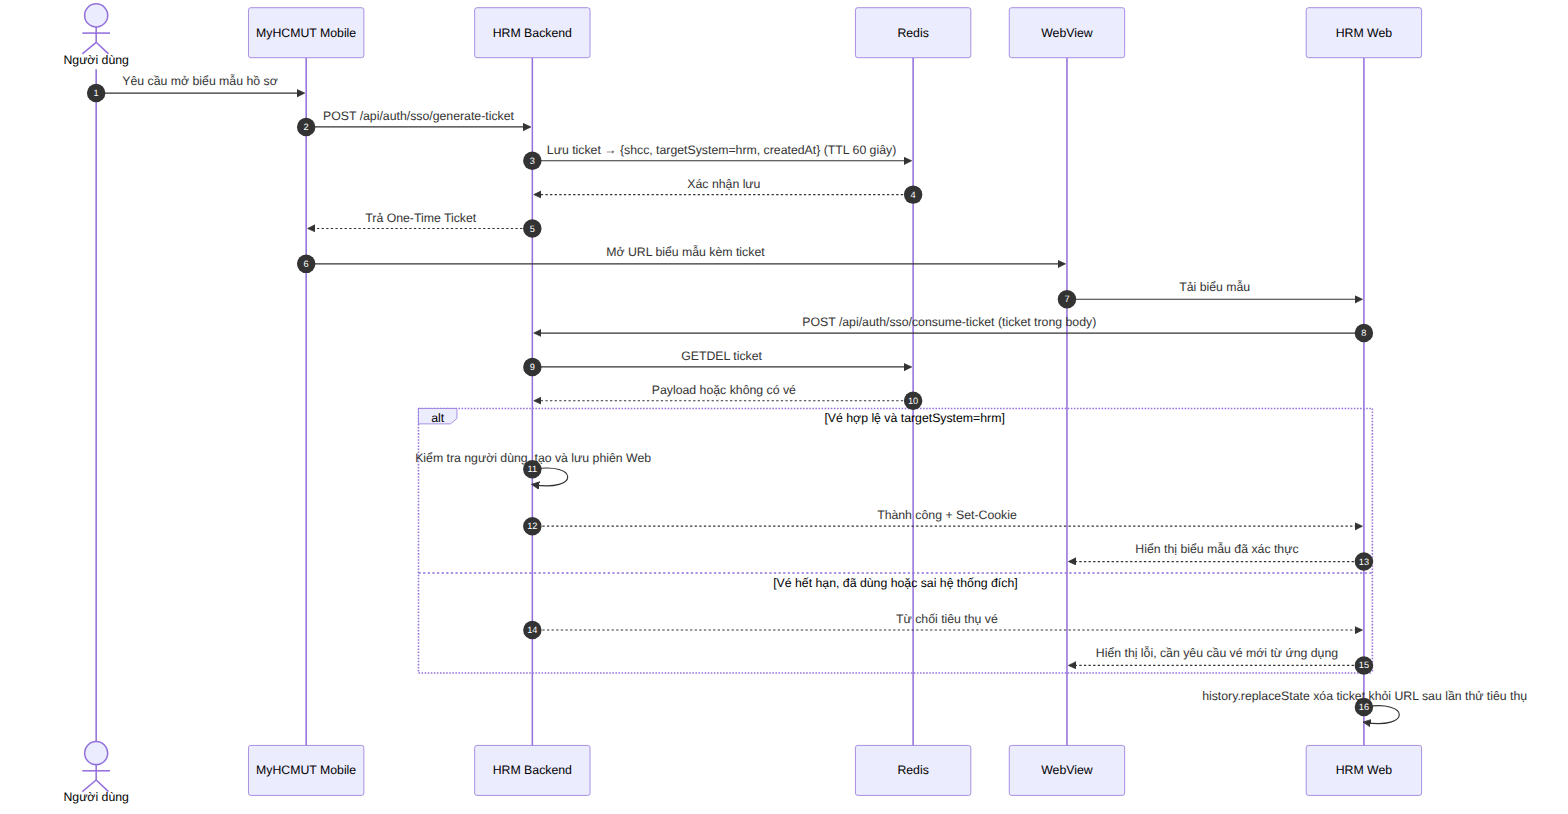
\includegraphics[width=0.78\linewidth,keepaspectratio]{image/architecture/chapter5-sso-flow.png}
    \caption[\textit{Luồng chuyển tiếp phiên làm việc từ MyHCMUT Mobile sang HRM Web bằng One-Time Ticket SSO}]{\textit{Luồng chuyển tiếp phiên làm việc từ MyHCMUT Mobile sang HRM Web bằng One-Time Ticket SSO}}
    \label{fig:sso_sequence}
\end{figure}

Việc tiêu thụ vé bằng \texttt{GETDEL} ngăn một vé hợp lệ bị tiêu thụ lại sau lần sử dụng đầu tiên. Tuy nhiên, vé vẫn xuất hiện tạm thời trên URL khi WebView được mở; thao tác xóa tham số sau đó không loại bỏ mọi khả năng lộ vé trước thời điểm này. Khi vé hết hạn hoặc đã được sử dụng, người dùng cần khởi tạo lại luồng chuyển tiếp từ ứng dụng để nhận vé mới.

Trong phạm vi phiên bản hiện tại, WebView được sử dụng để mở biểu mẫu HRM Web; ứng dụng chưa hỗ trợ truy cập các chức năng iOffice thông qua WebView, dù phía iOffice đã có thành phần tiêu thụ vé trong mã nguồn.

\subsection{Tích hợp thông báo}
\label{subsec:tich_hop_thong_bao}

MyHCMUT Mobile sử dụng Firebase Cloud Messaging (FCM) để tiếp nhận thông báo đẩy từ các hệ thống nghiệp vụ. HRM và iOffice duy trì cơ chế tạo và xử lý thông báo riêng; thông báo đẩy từ hai hệ thống được chuyển đến thiết bị thông qua FCM. Phần này tập trung vào điểm tích hợp với ứng dụng; việc xử lý nghiệp vụ và lưu trữ thông báo tại từng hệ thống nguồn không được mô tả chi tiết. Sơ đồ điểm tích hợp và luồng xử lý điều hướng thông báo được thể hiện trong Hình~\ref{fig:notification_routing_flow}.

\begin{figure}[H]
    \centering
    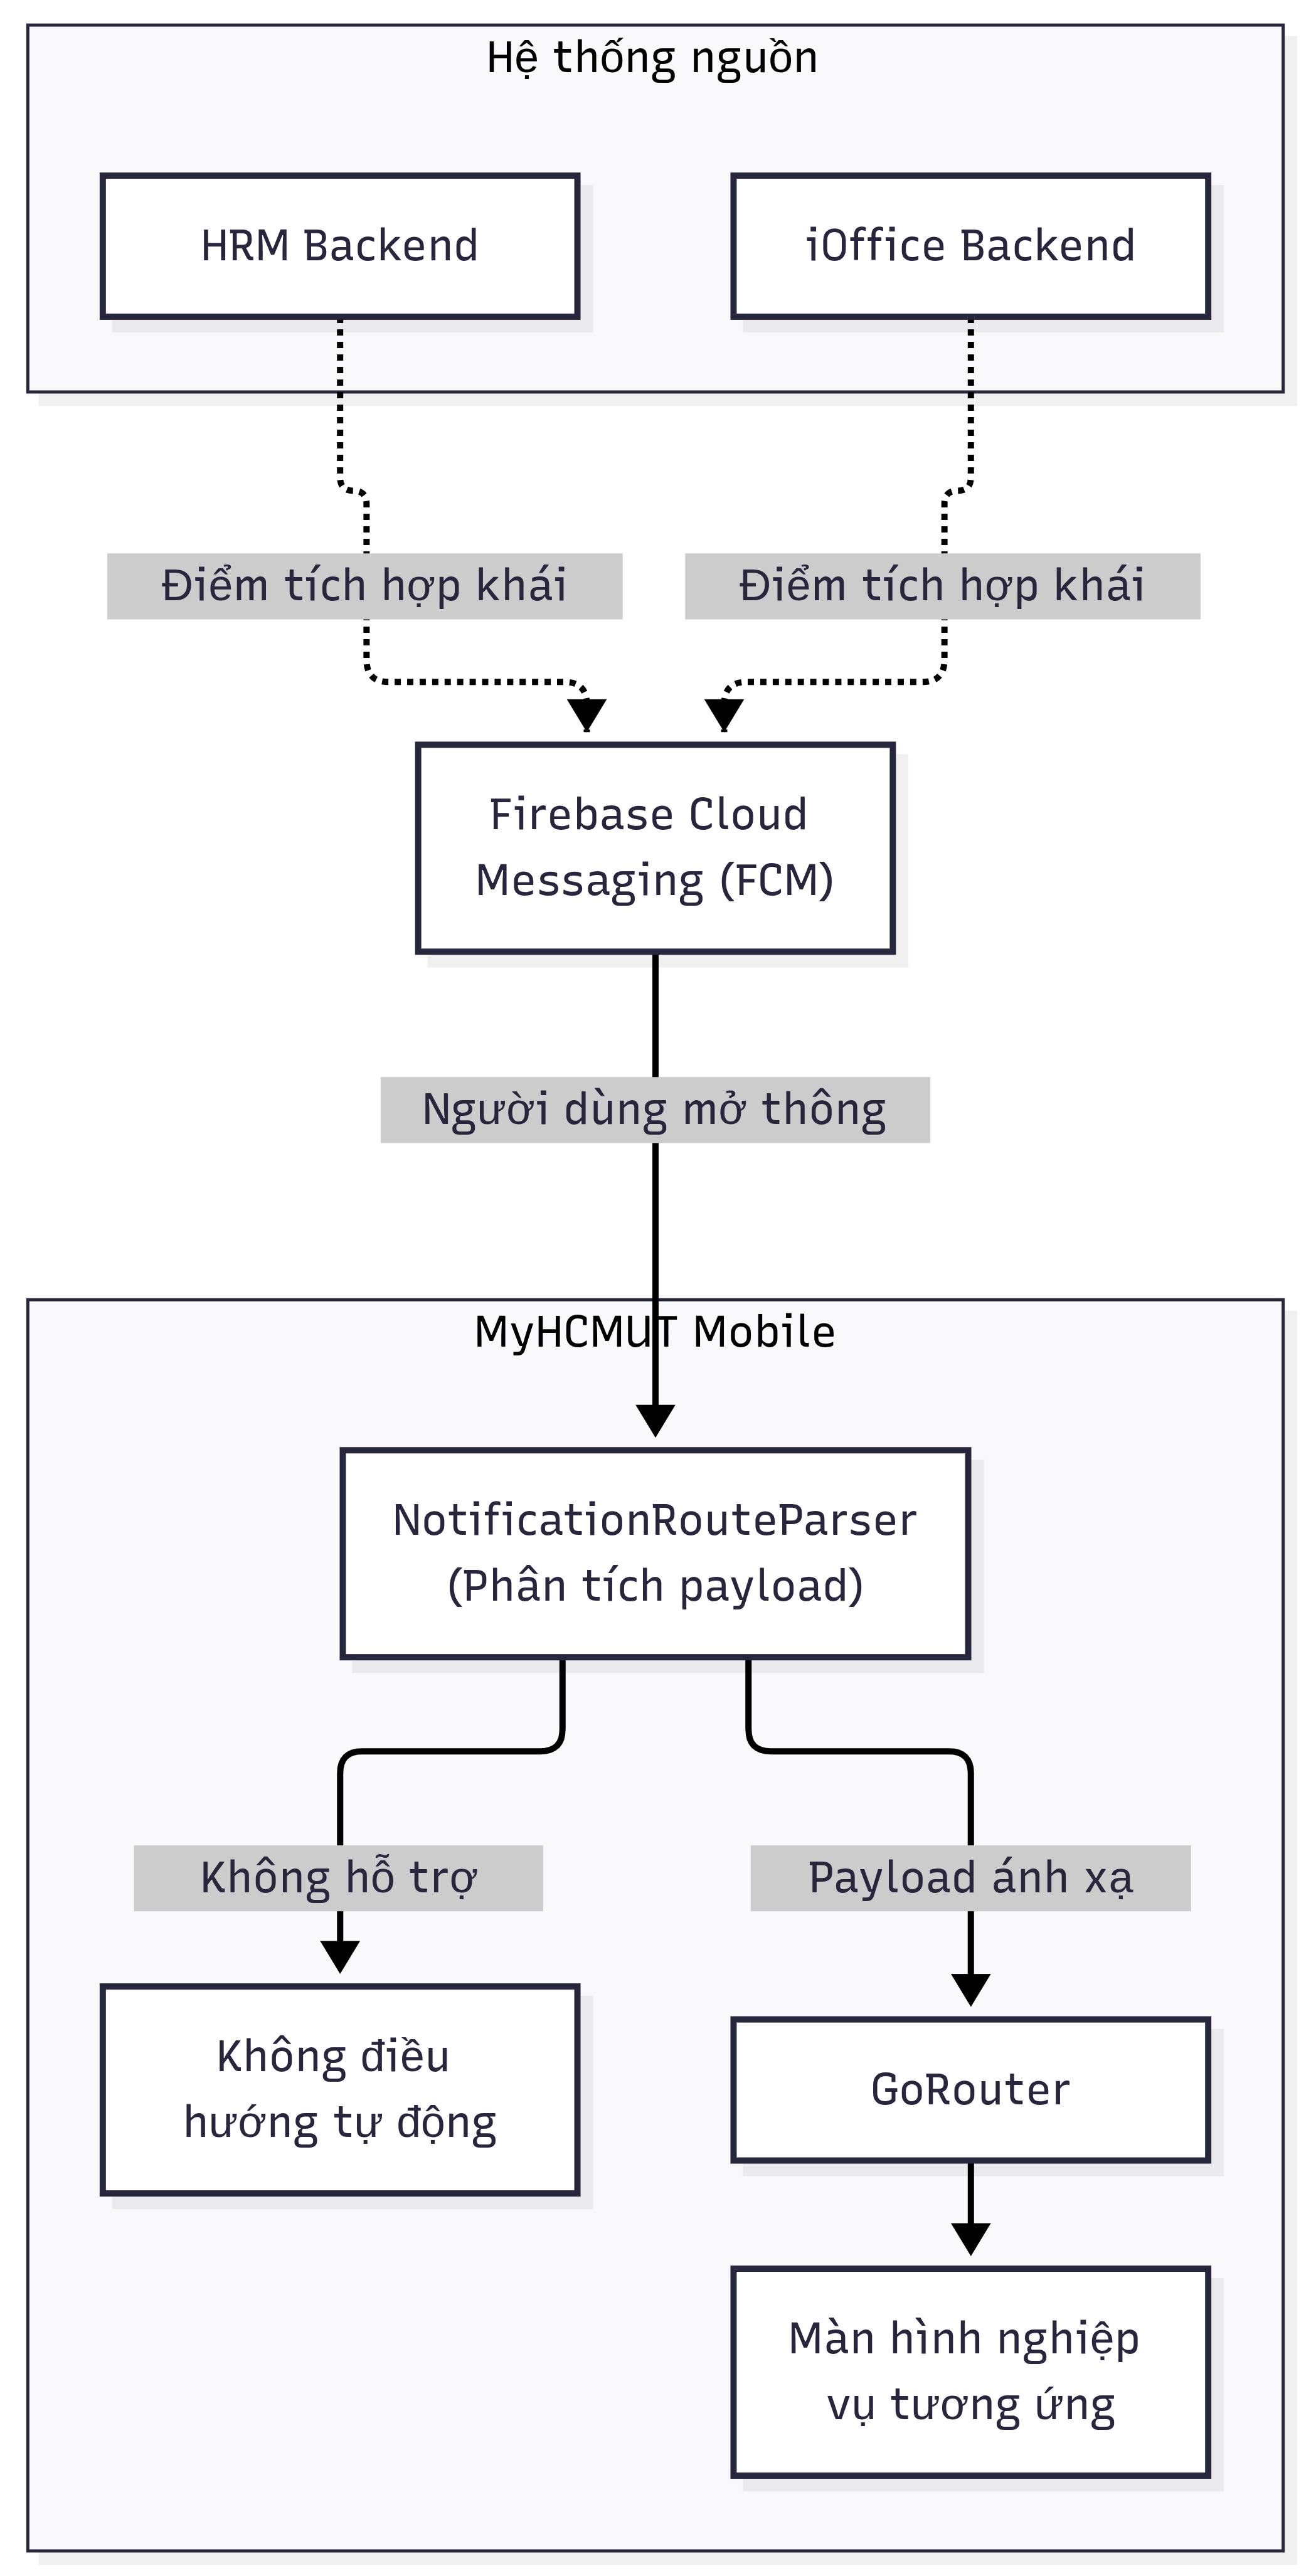
\includegraphics[width=0.46\linewidth,keepaspectratio]{image/architecture/notification-flow.png}
    \caption[\textit{Sơ đồ khái quát điểm tích hợp thông báo từ HRM và iOffice đến ứng dụng di động}]{\textit{Sơ đồ khái quát điểm tích hợp thông báo từ HRM và iOffice đến ứng dụng di động}}
    \label{fig:notification_routing_flow}
\end{figure}

Khi người dùng mở thông báo, ứng dụng đọc thông tin điều hướng trong payload, gồm \texttt{source}, \texttt{entityType}, \texttt{entityId}, \texttt{isApproval} hoặc \texttt{targetLink}, để xác định chức năng và đối tượng nghiệp vụ. Nếu ánh xạ được đích điều hướng, ứng dụng dùng GoRouter để mở màn hình liên quan. Nếu payload không ánh xạ được đến route được hỗ trợ, ứng dụng không thực hiện điều hướng tự động.

FCM là kênh chuyển thông báo đẩy, không thay thế dữ liệu nghiệp vụ do backend quản lý. Việc gửi thông báo không đồng nghĩa với việc thiết bị chắc chắn đã nhận hoặc người dùng đã xem thông báo.

\subsection{Tổng hợp lịch công tác và cập nhật điểm danh}
\label{subsec:tich_hop_lich_da_nguon}

\textbf{Tổng hợp lịch công tác.} Ứng dụng xây dựng lịch hiển thị chung từ dữ liệu của iOffice và HRM mà không tạo bảng lịch hợp nhất hoặc quan hệ trực tiếp giữa hai cơ sở dữ liệu. iOffice cung cấp danh sách lịch chính; dữ liệu nghỉ phép và đi công tác từ HRM được ánh xạ sang mô hình \texttt{ScheduleItem}. Flutter hợp nhất các danh sách và sắp xếp kết quả để hiển thị trên cùng giao diện.

Các yêu cầu lấy dữ liệu HRM được xử lý độc lập với nguồn lịch chính. Nếu API nghỉ phép hoặc đi công tác gặp lỗi, ứng dụng vẫn có thể hiển thị lịch lấy từ iOffice. Ngược lại, nếu API lịch chính của iOffice thất bại, provider hiện trả về trạng thái lỗi; ứng dụng chưa bảo đảm tiếp tục hiển thị lịch chỉ từ hai nguồn HRM trong trường hợp này. Để phân biệt các sự kiện HRM trong mô hình hiển thị, ứng dụng sử dụng quy ước định danh riêng, trong đó có ID âm. Quy ước này chỉ phục vụ xử lý tại Flutter, không làm thay đổi khóa chính hoặc cấu trúc dữ liệu của hệ thống nguồn.

\textbf{Cập nhật điểm danh cuộc họp.} Các thao tác điểm danh, báo vắng và hoàn tác được ứng dụng gửi đến iOffice Backend thông qua REST API. Sau khi trạng thái điểm danh thay đổi, iOffice Backend phát sự kiện Socket.IO để thông báo cho các thiết bị đang theo dõi lịch. Trong implementation hiện tại, sự kiện \texttt{scheduleCheckin} được sử dụng cho thao tác điểm danh và hoàn tác điểm danh, còn \texttt{scheduleAbsence} được sử dụng cho thao tác báo vắng.

Khi nhận được sự kiện, ứng dụng vô hiệu hóa trạng thái chi tiết lịch đang lưu và tải lại dữ liệu từ backend để cập nhật giao diện. REST API đảm nhiệm thực hiện thao tác nghiệp vụ, còn Socket.IO thông báo thay đổi trạng thái để các thiết bị đang theo dõi tải lại dữ liệu; trạng thái hiển thị được lấy từ phản hồi của backend. Hai cơ chế tích hợp lịch và điểm danh được tổng hợp trong Hình~\ref{fig:multi_source_schedule_flow}.

\begin{figure}[H]
    \centering
    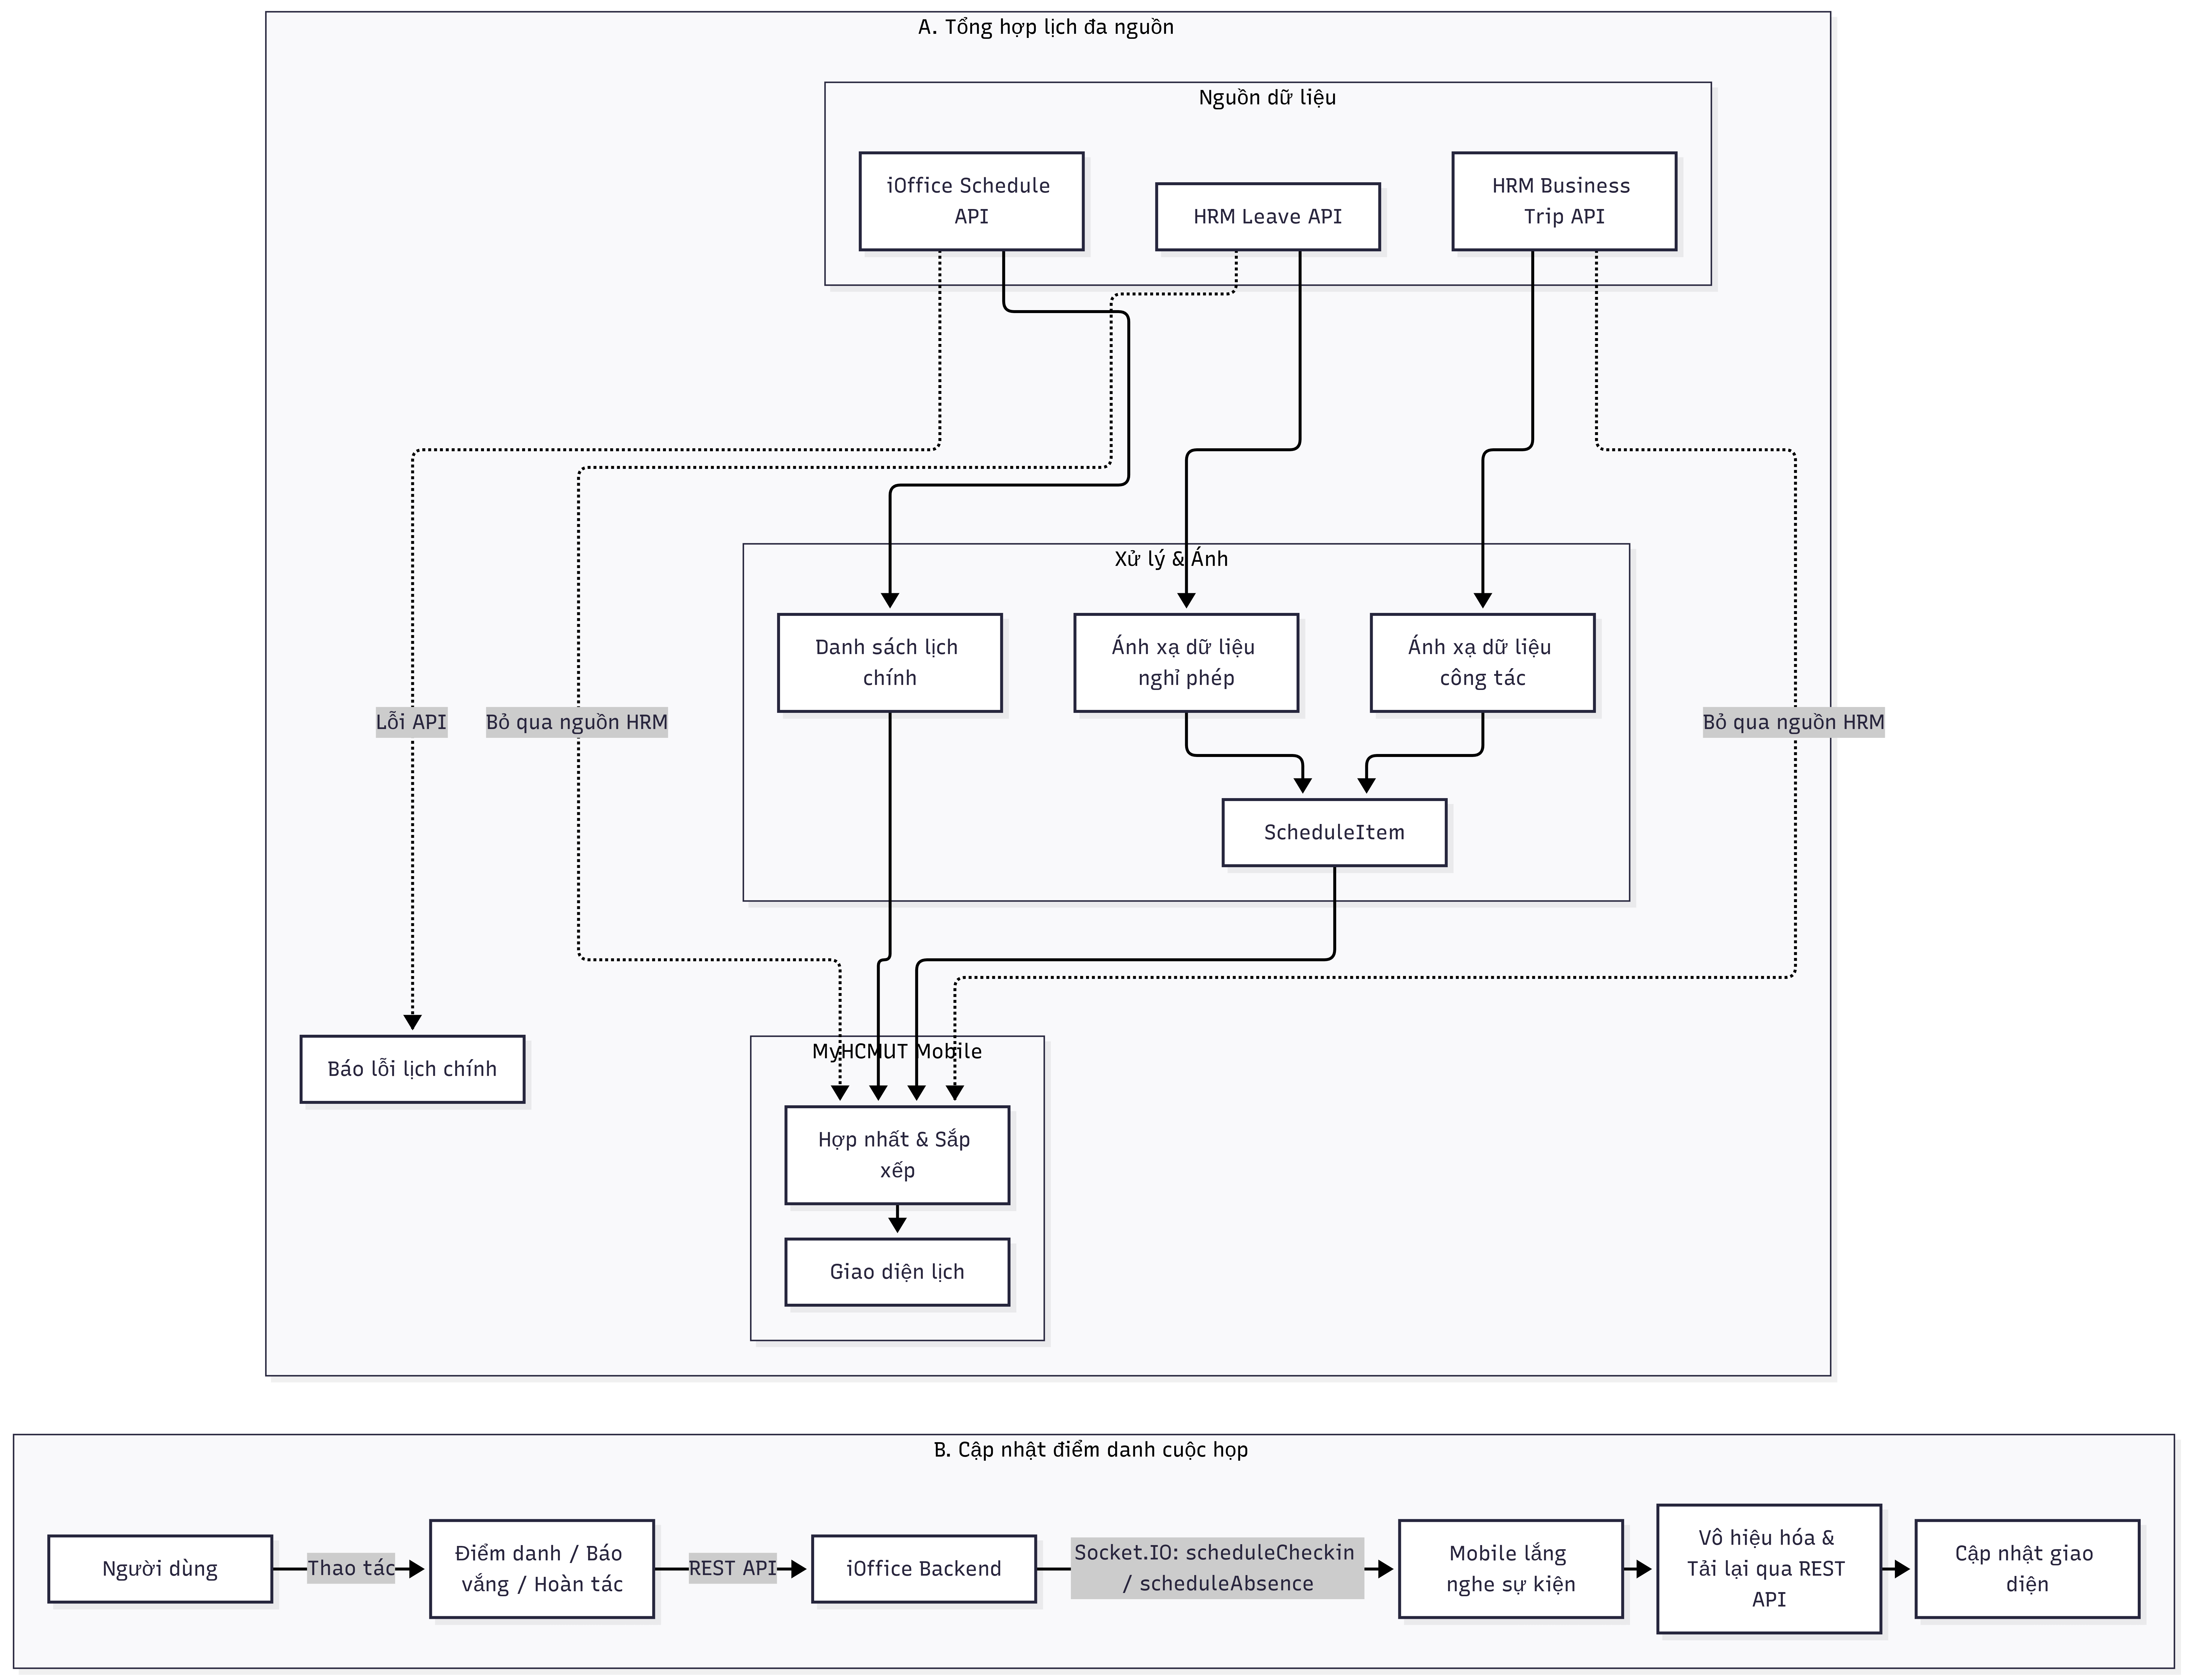
\includegraphics[width=\linewidth,keepaspectratio]{image/architecture/calendar-attendance.png}
    \caption[\textit{Tổng hợp lịch đa nguồn và cập nhật điểm danh cuộc họp}]{\textit{Tổng hợp lịch đa nguồn và cập nhật điểm danh cuộc họp}}
    \label{fig:multi_source_schedule_flow}
\end{figure}
